% !TeX root = ../../../main.tex

The theory of the strong  force, Quantum Chromodynamics, describes the proton
in terms of quarks and gluons. The proton is a state of two up quarks and one
down quark bound by gluons, but quantum theory predicts that in addition there
is an infinite number of quark-antiquark pairs.
%
Both light and heavy quarks, whose  mass is respectively smaller or bigger than
the mass of the proton, are  revealed inside the proton in high-energy
collisions.
%
However, it is unclear whether heavy quarks also exist as a part of the proton
wave-function, which is determined by non-perturbative dynamics and
accordingly unknown: so-called intrinsic heavy quarks~\cite{Brodsky:1980pb}.
It has been
argued for a long time that the proton could have a sizable intrinsic component
of the lightest  heavy quark, the charm quark.
Innumerable efforts to establish intrinsic charm in the
proton~\cite{Brodsky:2015fna} have remained inconclusive.
%
Here we provide evidence for intrinsic charm by exploiting a high-precision
determination of the quark-gluon content of the nucleon~\cite{Ball:2021leu}
based on machine learning and a large experimental dataset.
%
We disentangle the intrinsic charm component from charm-anticharm pairs arising
from high-energy radiation~\cite{Ball:2015tna}.
We establish the existence of intrinsic charm at the  $3\sigma$ level, with a
momentum distribution in remarkable agreement with model
predictions~\cite{Brodsky:1980pb,Hobbs:2013bia}.
%
We confirm these findings by comparing to very recent data on $Z$-boson
production with charm jets  from the LHCb experiment~\cite{LHCb:2021stx}. 

\section*{Main}

The foundational deep-inelastic scattering experiments at the SLAC linear collider
in the late 60s and early 70s demonstrated the presence inside the
proton of pointlike  constituents, soon identified with quarks, the
elementary particles that interact and are bound inside the proton by
gluons, the carriers of the strong  nuclear force.
%
It was rapidly clear, and confirmed in detail by subsequent studies,
that these pointlike constituents, collectively called ``partons'' by
Feynman~\cite{Feynman:1969wa}, include the up and down quarks that
carry the proton quantum numbers, but also gluons, as well
as an infinite number of pairs of quarks and their
antimatter counterparts, antiquarks.
%
The description of electron-proton and proton-proton collisions at high
momentum transfers in terms of collisions between partons is now
rooted in the theory of Quantum  Chromodynamics (QCD), and it provides
the basis
of modern-day precision phenomenology at proton accelerators such as
the Large Hadron Collider
(LHC) of CERN~\cite{Gao:2017yyd} as well
as for future facilities including the
EIC~\cite{AbdulKhalek:2021gbh},
the FPF~\cite{Feng:2022inv},
and  
neutrino telescopes~\cite{IceCube-Gen2:2020qha}.

Knowledge of the structure of the proton, which is necessary in order
to obtain
quantitative prediction for physics processes at the LHC and other
experiments, is encoded in
the distribution of  momentum carried by partons of each type
(gluons, up quarks, down quarks, up antiquarks, etc):
parton distribution functions (PDFs).
%
These PDFs could be in principle
computed from first principles, but in
practice even their determination from numerical
simulations~\cite{Constantinou:2020hdm} is extremely challenging.
%
Consequently,  the only 
strategy currently available for obtaining the
reliable determination of the proton PDFs which is required to evaluate LHC
predictions is empirical, through the global analysis of
data for which precise theoretical predictions and experimental
measurements are available, so that the PDFs are the only
unknown~\cite{Gao:2017yyd}.

While this successful framework has by now been worked through in great detail, several key open questions remain open.
%
One of the most controversial of these concerns the treatment of
so-called heavy quarks, i.e.\ those whose mass is greater than that of
the proton ($m_p=0.94$~GeV). Indeed, virtual quantum effects and
energy-mass considerations suggest that the three light quarks and
antiquarks (up, 
down, and strange) should all be present in the proton
wave-function.
%
Their PDFs are therefore surely determined by the low-energy
dynamics that controls the nature of the proton as a bound
state.
%
However, it is a well-known fact~\cite{DeRoeck:2011na,
  Kovarik:2019xvh,Gao:2017yyd,Rojo:2019uip}
that in high enough energy collisions all species of quarks can be
excited and hence observed
inside the proton, so their PDFs are nonzero.
%
This excitation
follows from standard QCD radiation and it can be computed accurately
in perturbation theory.

But then the question arises: do heavy quarks also contribute to the
proton wave-function? Such a contribution is called ``intrinsic'', to
distinguish it from that computable in
perturbation theory, which originates from QCD radiation.
%
Already since the dawn of QCD, it
was argued that all kinds of intrinsic heavy quarks must be
present in the
proton wave-function~\cite{Brodsky:1984nx}.
%
In particular, it was
suggested~\cite{Brodsky:1980pb}
that the intrinsic component could be non-negligible for the
charm quark, whose mass ($m_c\simeq 1.51$ GeV) is of the same order of
magnitude as the mass of the proton.

This question has remained highly controversial, and indeed recent
dedicated studies have resulted in disparate claims,
from excluding momentum fractions carried by intrinsic  charm larger than 0.5\% at the 4$\sigma$
level~\cite{Jimenez-Delgado:2014zga} to allowing up to a 2\% charm momentum
fraction~\cite{Hou:2017khm}.
%
A particularly delicate issue in this context is that of
separating the radiative component: finding that the charm PDF
is nonzero at a low scale is not sufficient to argue that intrinsic charm
has been identified.

Here we present a resolution of this four-decades-long conundrum
by providing unambiguous evidence for intrinsic charm  in the proton.
%
This is achieved by means of a determination of the charm
PDF~\cite{Ball:2021leu} from the most extensive hard-scattering 
global dataset analyzed to date, using state-of-the-art perturbative
QCD calculations~\cite{Heinrich:2020ybq}, adapted to accommodate the possibility of massive quarks inside the proton~\cite{Forte:2010ta,Ball:2015dpa,Ball:2015tna}, and sophisticated machine 
learning (ML)
techniques~\cite{Ball:2016neh,Ball:2017nwa,Ball:2021leu}. This
determination is performed at next-to-next-to-leading-order (NNLO) in an
expansion in powers of the strong coupling, $\alpha_s$, which
represents the precision frontier for collider phenomenology.
%

The charm PDF determined in this manner includes a 
radiative component, and
indeed it depends on the resolution scale: it is 
given in a four-flavor-number scheme (4FNS), in which up, 
down, strange and charm quarks are subject to  perturbative
radiative corrections and mix with each other and the gluon as the
resolution is increased.
%
The
intrinsic charm component can be disentangled from it as follows.
%
First, we
note that in the absence of an intrinsic component, the initial
condition for the charm PDF is determined using perturbative matching
conditions~\cite{Collins:1986mp}, computed  up to NNLO in~\cite{pdfnnlo},
and recently (partly) extended up to N$^3$LO~\cite{Bierenbaum:2009zt,Bierenbaum:2009mv,Ablinger:2010ty,Ablinger:2014vwa,Ablinger:2014uka,Behring:2014eya,Ablinger_2014,Ablinger:2014nga,Blumlein:2017wxd}.
%
These matching conditions 
determine the charm PDF in terms of the PDFs of the
three-flavor-number-scheme (3FNS), in which only the three lightest quark 
flavors are radiatively corrected.
%
Hence this perturbative charm PDF is
entirely determined in terms of the three light quarks and antiquarks
and the gluon.
%
However, the 3FNS charm quark PDF needs not
vanish: in fact, if the charm quark PDF in the 4FNS is freely
parametrized and thus determined from the data~\cite{Ball:2015tna},
the matching conditions can be inverted.
%
The 3FNS charm PDF
thus obtained is then by definition the intrinsic charm PDF: indeed, in
the absence of intrinsic charm it would vanish~\cite{Ball:2015dpa}. 
Thus unlike the 4FNS charm PDF, that
includes both an intrinsic and a radiative
component, the 3FNS charm
PDF is purely intrinsic.
%
In this work we have performed this inversion at
NNLO~\cite{pdfnnlo} as well as at N$^3$LO~\cite{Bierenbaum:2009zt,Bierenbaum:2009mv,Ablinger:2010ty,Ablinger:2014vwa,Ablinger:2014uka,Behring:2014eya,Ablinger_2014,Ablinger:2014nga,Blumlein:2017wxd},
which as we shall see provides a handle on the perturbative uncertainty of the NNLO result.

Our starting point is the NNPDF4.0 global
analysis~\cite{Ball:2021leu}, which provides a determination of
the sum of the charm and
anticharm PDFs, namely  $c^+(x,Q)\equiv c(x,Q)+\bar  c(x,Q)$, in the
4FNS. 
This can be viewed 
as a probability density in $x$, the fraction of the proton momentum
carried by charm, in the sense that the integral over all 
values of $0\le x\le1$ of 
$xc^+(x)$ is equal to  the fraction of
the proton momentum carried by charm quarks, though note that PDFs are
generally not necessarily positive-definite. 
%
Our result for  the 4FNS $xc^+(x,Q)$  at
the charm mass scale, $Q=m_c$ with $m_c=1.51$ GeV, 
is displayed in Fig.~\ref{fig:ic/charm_content_3fns}~(left).
%
%
The ensuing intrinsic charm is determined from it
by transforming to the 3FNS using
NNLO matching.
%
This result is also shown 
in Fig.~\ref{fig:ic/charm_content_3fns}~(left).
The bands  indicate the 68\% confidence level (CL) interval
associated with the PDF uncertainties  (PDFU) in each case.  Henceforth, we will refer to
the  3FNS $xc^+(x,Q)$ PDF as the
intrinsic charm PDF. 

%%%%%%%%%%%%%%%%%%%%%%%%%%%%%%%%%%%%%%%%%%%%%%%%%%%%%%%%%%%%%%%%%%%
\begin{figure}[h]
  \begin{center}
    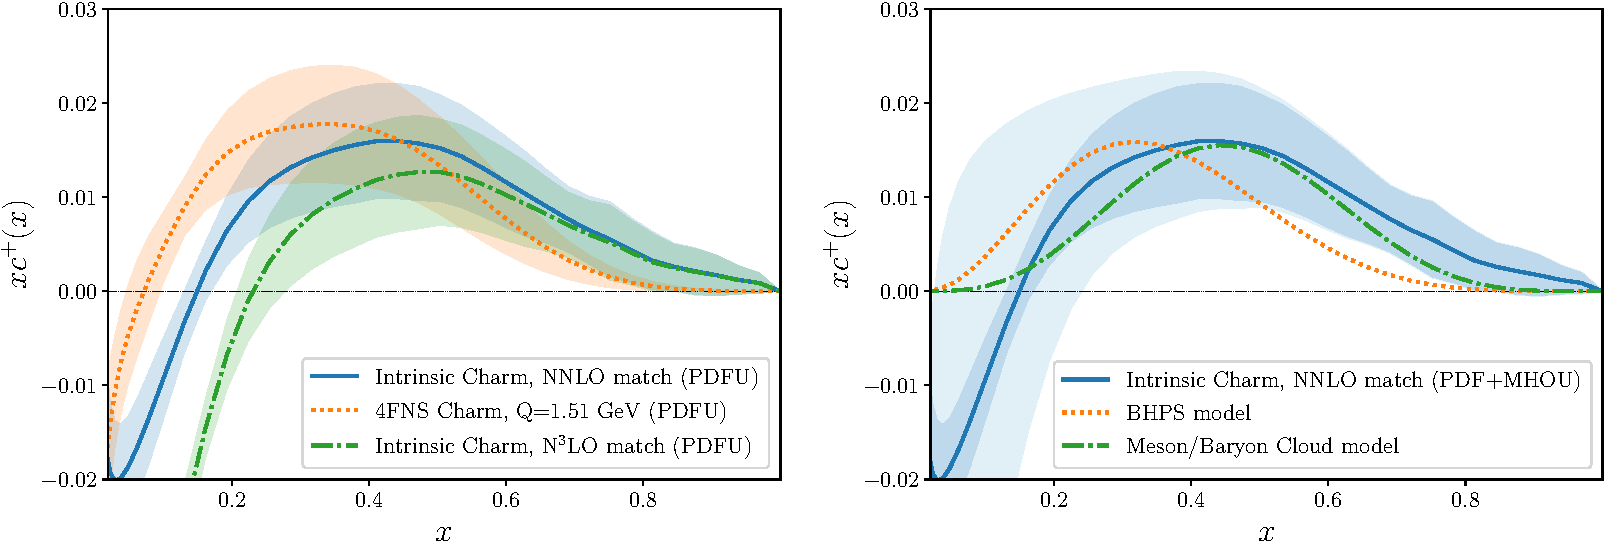
\includegraphics[width=0.99\linewidth]{ch-ic/Fig1.pdf}
    \caption{\small  \textbf{ The intrinsic charm PDF
      and comparison with models}.
%
      Left: the purely
      intrinsic (3FNS) result (blue)
      with PDF uncertainties only, compared to the 4FNS PDF, that
      includes both an intrinsic and radiative
      component,   at
      $Q=m_c=1.51$ GeV (orange). The purely intrinsic (3FNS)
      result obtained using N$^3$LO matching is also shown (green).
      %
      Right: the purely
      intrinsic (3FNS)
      final result with total uncertainty (PDF+MHOU), with the PDF
      uncertainty indicated as a dark shaded band;
the predictions from the original 
BHPS model~\cite{Brodsky:1980pb} and from the more recent meson/baryon
      cloud model~\cite{Hobbs:2013bia} are also shown for comparison
      (dotted and dot-dashed curves respectively).
         \label{fig:ic/charm_content_3fns} }
\end{center}
\end{figure}
%%%%%%%%%%%%%%%%%%%%%%%%%%%%%%%%%%%%%%%%%%%%%%%%%%%%%%%%%%%%%%%%%%%%%%

The intrinsic (3FNS) charm PDF
displays a characteristic valence-like
 structure at large-$x$ peaking at $x\simeq 0.4$.
%
 While intrinsic charm is found to be small in absolute terms
 (it contributes less than 1\% to the proton  total momentum),
 it is significantly different from zero.
%
 Note that the transformation to the 3FNS has little effect on the peak region,
 because there is almost no charm radiatively generated at such large values of $x$: in
 fact, a very similar valence-like peak is already found in the 4FNS calculation.

Because at the charm mass scale the strong coupling $\alpha_s$ is rather
large, the perturbative expansion converges slowly.
%
In order to
estimate the effect of missing higher order uncertainties (MHOU), we
have also performed the transformation from the 4FNS NNLO charm PDF
determined from the data to the 3FNS (intrinsic) charm PDF at one
order higher, namely at N$^3$LO. 
%
The result is also shown
Fig.~\ref{fig:ic/charm_content_3fns} (left). Reassuringly, the intrinsic
valence-like structure is unchanged.
%
On the other hand, it is clear that for
$x\lsim 0.2$ perturbative uncertainties become very large.
%
We can estimate  the total uncertainty on our determination
of intrinsic charm by adding in quadrature the PDF uncertainty and a
MHOU estimated from the shift between the result found using NNLO
and N$^3$LO matching.

This procedure leads to our final result for intrinsic charm and its total
uncertainty, shown in Fig.~\ref{fig:ic/charm_content_3fns} (right).
%
The intrinsic charm PDF is found to be compatible with zero for
$x\lsim 0.2$: the negative trend 
seen  in Fig.~\ref{fig:ic/charm_content_3fns} with PDF uncertainties only 
becomes 
compatible with zero upon inclusion of  theoretical
uncertainties. However, at
larger $x$ even with theoretical uncertainties
the intrinsic charm PDF
 differs 
from zero by about 2.5 standard deviations ($2.5\sigma$) in the peak region.
%
This result  is stable upon variations of dataset, methodology (in
particular the PDF  parametrization basis) and Standard Model
parameters (specifically the charm mass),
as demonstrated in the Supplementary Information (SI) Sects.~\ref{app:ic/charm_stability_4fns}
and~\ref{app:ic/charm_stability_3fns}. 

Our determination of intrinsic charm can be compared to theoretical expectations.
%
Subsequent to the
original intrinsic charm model of~\cite{Brodsky:1980pb} (BHPS
model),
a variety of other models were  
proposed~\cite{Hoffmann:1983ah,Pumplin:2005yf,Paiva:1996dd,Steffens:1999hx,Hobbs:2013bia},
see~\cite{Brodsky:2015fna} for a review.
%
Irrespective of their specific details, most models predict a valence-like
structure at large $x$ 
with a maximum located  between $x\simeq 0.2$ and $x\simeq 0.5$, and a
vanishing intrinsic component for
$x\lsim 0.1$.
%
In Fig.~\ref{fig:ic/charm_content_3fns}~(right) we compare our result to
the original BHPS model and to the more recent meson/baryon cloud model of~\cite{Hobbs:2013bia}.

As these models predict only the shape of the
intrinsic charm distribution, but not 
its overall normalization, we have normalized them by requiring
that they reproduce the same 
charm momentum fraction as our determination.
%
We find remarkable agreement between the shape of our 
determination and the model predictions.
%
In particular, we reproduce  the presence and location of the large-$x$ valence-like peak
structure (with  better agreement, of marginal statistical significance, with
the meson/baryon cloud calculation),  and the vanishing of 
intrinsic charm at small-$x$.
%
The fraction of the proton momentum carried by charm quarks that we
obtain from our analysis, 
used in this comparison to models,  is $\left( 0.62 \pm 0.28\right) \%$
including PDF uncertainties only (see
SI Sect.~\ref{app:ic/charm_mom_frac} for details).
%
However, the uncertainty
upon inclusion of MHOU greatly increases, and we obtain
$\left( 0.62 \pm 0.61\right) \%$, due to the contribution from the small-$x$
region, $x\lsim 0.2$, where the MHOU is very large, see
Fig.~\ref{fig:ic/charm_content_3fns}~(right).
%
%
Note that in most previous
analyses~\cite{Hou:2017khm} (see SI Sect.~\ref{app:ic/ct}) intrinsic charm models (such as the BHPS
model) are fitted to the data, with only the momentum fraction left as
a free parameter.

We emphasize that in our analysis the charm PDF is entirely
determined by the experimental data included in the PDF determination.
The data with the most impact on charm are from recently measured LHC
processes, which are both accurate and precise.
%
Since these measurements are made at high scales, the corresponding
hard cross-sections can be reliably computed in QCD perturbation theory.

Independent evidence for intrinsic charm
is provided by the very recent LHCb measurements of $Z$-boson production
in association with charm-tagged jets in the forward
region~\cite{LHCb:2021stx}, which were not included in our baseline dataset.
%
This process, and specifically the ratio $\mathcal{R}_j^c$
of charm-tagged jets normalized to flavor-inclusive jets,
is directly sensitive to the charm PDF~\cite{Boettcher:2015sqn}, and
with LHCb kinematics also
in the kinematic region  where the  intrinsic component is relevant.
%
Following~\cite{Boettcher:2015sqn,LHCb:2021stx}, we have 
evaluated $\mathcal{R}_j^c$ at NLO~\cite{Alioli:2010xd,Sjostrand:2007gs}  
(see  SI Sect.~\ref{sec:ic/zcharm} for details), both with our default PDFs
that include intrinsic charm, and also with an independent PDF determination in
which intrinsic charm is constrained to vanish 
identically, so charm is determined by perturbative matching
(see SI Sect.~\ref{app:ic/consistency}).

%%%%%%%%%%%%%%%%%%%%%%%%%%%%%%%%%%%%%%%%%%%%%%%%%%%%%%%%%%%%%%%%%%%
\begin{figure}[htbp]
  \begin{center}
    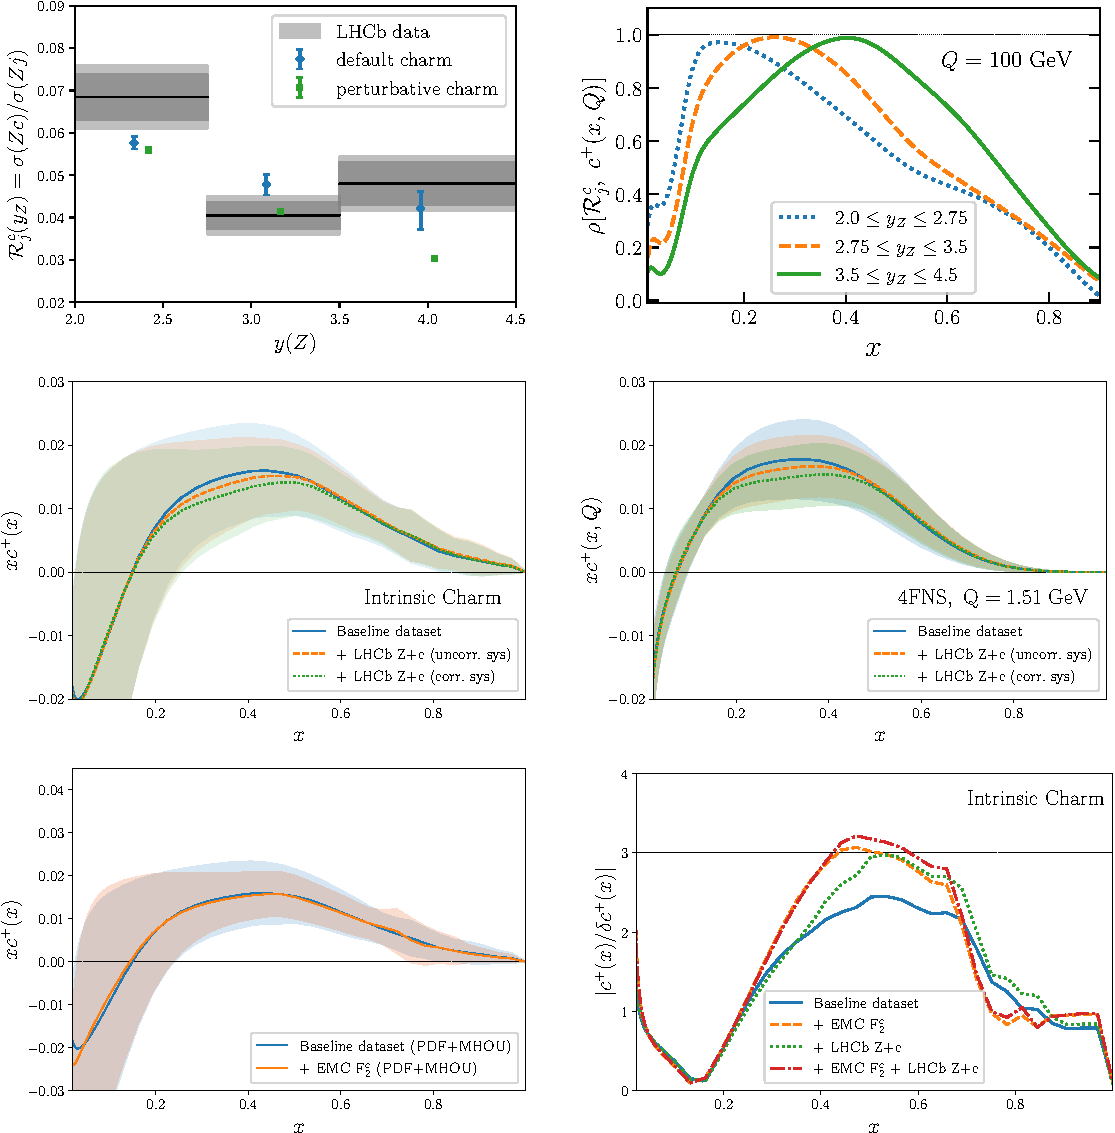
\includegraphics[width=0.99\linewidth]{ch-ic/Fig2.pdf}
     \caption{\small
       \textbf{ Intrinsic charm and $Z+$charm production at LHCb.}
       %
       Top left: the LHCb measurements of $Z$ boson production
      in association with charm-tagged jets, $\mathcal{R}_j^c$, at $\sqrt{s}=13$ TeV,  compared with
      our default prediction which includes an intrinsic charm component,
      as well as with a variant in which we impose the
      vanishing of the intrinsic charm component.
      %
       The thicker (thinner) bands in the LHCb data indicate the statistical
      (total) uncertainty, while the theory predictions include both PDF and MHO uncertainties.
      %
      Top right: the correlation coefficient between
     the  charm PDF at $Q=100$ GeV in NNPDF4.0
      and the LHCb measurements of $\mathcal{R}_j^c$ 
     for the three $y_Z$ bins.
      %
     Center: the charm PDF
     in the 4FNS (right) and the intrinsic (3FNS) charm PDF (left)
     before and after inclusion of the LHCb $Z$+charm data.
     %
     Results are shown
     for both experimental correlation models discussed in the text.
     %
     Bottom left: the intrinsic charm PDF before and after inclusion
     of the EMC charm structure function data.
     %
     Bottom right: the statistical significance of the
     intrinsic charm PDF in our baseline analysis, compared to the results
     obtained also including either the LHCb $Z$+charm (with uncorrelated
     systematics) or the EMC
     structure function data, or both.
  \label{fig:ic/Zc} }
\end{center}
\end{figure}
%%%%%%%%%%%%%%%%%%%%%%%%%%%%%%%%%%%%%%%%%%%%%%%%%%%%%%%%%%%%%%%%%%%%%%

In Fig.~\ref{fig:ic/Zc}~(top left) we compare the LHCb measurements of $\mathcal{R}_j^c$, provided
in three bins of the $Z$-boson rapidity
$y_Z$, with the theoretical predictions
 based on both our default PDFs as well as the PDF set in
 which we impose the vanishing of intrinsic charm.
 %
 In Fig.~\ref{fig:ic/Zc}~(top right)
we also display the  correlation coefficient between
 the  charm PDF at $Q=100$ GeV 
 and the observable  $\mathcal{R}_j^c$, demonstrating how this observable
 is highly
 correlated to charm in a localized
 $x$ region that depends on the rapidity bin.
 %
 It is clear that
 our prediction is in excellent agreement with the LHCb measurements, while in the
 highest rapidity bin, which is highly correlated to the charm PDF in
 the region of the observed valence peak $x\simeq 0.45$, the prediction
 obtained by imposing the vanishing of intrinsic charm undershoots the
 data at the $3\sigma$ level.
%
 Hence this measurement provides
 independent direct evidence in support of our result.

 We have also determined the impact of these LHCb $Z$+charm measurements on the
charm PDF.
%
Since the experimental covariance matrix is not available,
we have considered two limiting scenarios in which the total
systematic uncertainty is either completely uncorrelated 
($\rho_\textrm{ sys}=0$) or fully correlated  ($\rho_\textrm{ sys}=1$) between
 rapidity bins. The charm PDF in the 4FNS before and after
inclusion of the LHCb data (with either correlation model), and the intrinsic
charm PDF obtained from it, are displayed in
Fig.~\ref{fig:ic/Zc}~(center left and right respectively).
%
The bands account for both PDF and MHO uncertainties.
%
The results show full consistency: inclusion of the LHCb  $\mathcal{R}_j^c$ data leaves
the intrinsic charm PDF unchanged, while moderately reducing the
uncertainty on it.

In the past, the main indication for  intrinsic charm came from EMC data~\cite{Aubert:1982tt} on deep inelastic scattering with charm in the final state~\cite{Harris:1995jx}.
%
These data are relatively imprecise, their accuracy has often been questioned,
and they were taken at relatively low scales where radiative corrections are large.
%
For these reasons, we have not included them in our baseline
analysis.
%
However, it is interesting to assess the impact of
their inclusion.
%
Results are shown in 
Fig.~\ref{fig:ic/Zc}~(bottom left), where we display the
intrinsic charm PDF before and after inclusion of the EMC data.
%
Just
like in the case of the LHCb data we find full consistency: unchanged
shape and a moderate reduction of uncertainties.

We can summarize our results  through their so-called local statistical
significance, namely, the size of the intrinsic charm PDF
in units of its total uncertainty.
%
This displayed  in Fig.~\ref{fig:ic/Zc}~(bottom right) for our default determination of
intrinsic charm, as well as after inclusion of either the LHCb $Z$+charm or the
EMC data, or both.
%
We find a local significance for intrinsic charm at the $2.5\sigma$ level
in the region $0.3 \lsim x \lsim 0.6$.
%
This is increased to about
$3\sigma$ by the inclusion of either the EMC or the LHCb
data, and above if they are both included.
%
The similarity of the impact of the EMC and LHCb measurements is
especially remarkable in view of the fact that they involve very
different physical processes and energies.

In summary, in this work we have presented
long-sought evidence for intrinsic charm quarks in the proton.
%
Our findings
close a fundamental open question
in the understanding of nucleon structure that has been hotly
debated by  particle and nuclear physicists for the last 40 years.
%
By carefully disentangling the perturbative component,
we obtain unambiguous evidence for intrinsic charm, 
which turns out to be in qualitative agreement with
the expectations from model calculations.
%
Our determination of the charm PDF, driven by indirect constraints from the 
latest high-precision LHC data, is perfectly
consistent with direct constraints both from EMC charm production
data taken forty years  
ago, and with very recent  $Z$+charm production data in the
forward region from LHCb.
%
Combining all data, we find
local significance for intrinsic charm in the large-$x$
region just above the  $3\sigma$ level.
%
Our results motivate
further dedicated studies of intrinsic charm through a wide range
of nuclear, particle and astro-particle physics experiments,
from the High-Luminosity LHC~\cite{Azzi:2019yne}
and the fixed-target programs of LHCb~\cite{LHCb:2018jry} and
ALICE~\cite{QCDWorkingGroup:2019dyv}, to
the  
Electron Ion Collider, AFTER~\cite{Hadjidakis:2018ifr},
the Forward Physics Facility~\cite{Anchordoqui:2021ghd},
and neutrino telescopes~\cite{Halzen:2016thi}.

%%%%%%%%%%%%%%%%%%%%%%%%%%%%%%%%%%%%%%%%%%%%%%%%%
%%%%%%%%%%%%%%%%%%%%%%%%%%%%%%%%%%%%%%%%%%%%%%%%%5

\subsection*{Acknowledgments}

We thank our colleagues of the NNPDF Collaboration
for many illuminating discussions concerning the charm PDF.
%
We are grateful to Johannes Bl\"umlein for communicating  \textsc{\small Mathematica}
code with the results
of~\cite{Bierenbaum:2009zt,Bierenbaum:2009mv,Ablinger:2010ty,Ablinger:2014vwa,Ablinger:2014uka,Behring:2014eya,Ablinger_2014,Ablinger:2014nga,Blumlein:2017wxd}, to
Jakob Ablinger for assistance
in the implementation of the $\mathcal{O}\left( \alpha_s^3 \right)$ calculation
of the heavy quark matching conditions, and to Silvia Zanoli
for sharing her \textsc{\small Mathematica} implementation with us.
%
%
We are grateful to Rhorry Gauld for discussions, assistance and sharing his \textsc{\small Pythia8} 
implementation for the calculation $Z$+charm production.
%
We thank Marco Guzzi and Pavel Nadolsky for discussions concerning intrinsic charm
in the CT family of global PDF fits, and Tim Hobbs and Wally Melnitchouk for providing
us with their predictions of the meson/baryon cloud model.
%
We are grateful to Tom Boettcher, Philip Ilten, and Michael Williams to assistance
with the LHCb $Z$+charm measurements.

\subsection*{Funding information}

S.~F., J.~C.-M., F.~H., A.~C., and K.~K. are supported by
the European Research Council under 
the European Union's Horizon 2020 research and innovation Programme
(grant agreement n.740006).
%
R.~D.~B. is supported by the U.K.
Science and Technology Facility Council (STFC) grant ST/P000630/1. 
%
J.~R. and G.~M. are partially supported by NWO (Dutch Research Council).
%
T.~G. is supported by NWO (Dutch Research Council) via an ENW-KLEIN-2 project.
%

\subsection*{Code and data availability}

The analysis presented in this work has been carried out using two
open-source software frameworks, \textsc{\small NNPDF} for the global
PDF determination and \textsc{\small EKO} for the calculation of the 3FNS charm.
%
These codes are publicly available from \url{https://docs.nnpdf.science/}
and \url{https://eko.readthedocs.io/} respectively.
%
Both the \textsc{\small LHAPDF} grids produced in this work and the version
of \textsc{\small EKO} with the respective run cards used are made available from
\url{http://nnpdf.mi.infn.it/nnpdf4-0-charm-study/}.

\subsection*{Author contributions}

As customary in high-energy physics, authors are listed
in alphabetical order.

J.~C.~M. is the main author of the new algorithm used in the NNPDF4.0
PDF determination.
A.~C., F.~H., and G.~M. developed the \textsc{\small EKO} code used
to evaluate the 3FNS charm PDF, and specifically G.~M. implemented the
matching conditions, with the help of K.~K. for the implementation of
some harmonic sums.
T.~G. performed the analysis of the LHCb $Z$+charm data.
R.~D.~B. and S.~F. designed the general procedure. J.~R. coordinated
the intrinsic charm determination and S.~F. supervised the whole
project. J.~R.~ and S.~F. wrote the paper and R.~D.~B. revised it.
All authors discussed the results and their implications.


% Methods section
\section*{Methods}
\label{sec:ic/methods}

The strategy adopted in this work in order to
determine the intrinsic charm content of the proton is 
based on the following
observation.
%
The assumption that there is no intrinsic charm
amounts to the assumption
that all 4FNS PDFs are determined~\cite{Collins:1986mp} using
perturbative matching conditions~\cite{pdfnnlo} in terms of 
3FNS PDFs
that do not include
a charm PDF.
%
However, these perturbative matching conditions are
actually given by a square matrix that also includes a 3FNS charm
PDF.
%
So the assumption of no intrinsic charm amounts to the assumption
that if the 4FNS PDFs are transformed back to the 3FNS, the 3FNS charm
PDF is found to vanish. Hence, intrinsic charm is by definition the
deviation from zero of the 3FNS charm PDF~\cite{Ball:2015dpa}. Note
that whereas the 3FNS charm PDF is purely intrinsic, while the 4FNS
charm PDF includes both an intrinsic and a perturbative
 radiative component, the
4FNS intrinsic component is not equal to the 3FNS charm PDF, since
matching conditions reshuffle all PDFs among each other. 

Intrinsic charm can then be determined through the following two steps,
summarized in Fig.~\ref{fig:ic/strategy}. 
First, all the PDFs, including the charm PDF, are parametrized 
in the 4FNS at an input scale $Q_0$ and evolved 
using NNLO perturbative QCD to   $Q \not = Q_0$.
%
These evolved PDFs can be used to 
compute physical cross-sections, also at NNLO, which then are
compared to a global dataset of experimental measurements.
%
The result of this first step in our procedure is 
a Monte Carlo (MC) representation
of the probability distribution for the 4FNS PDFs at the input
parametrization scale $Q_0$.

Next, this 4FNS charm PDF is transformed to the 3FNS at some scale matching scale
$Q_c$.
%
Note that the choice of both $Q_0$ and $Q_c$ are immaterial. The former
because perturbative evolution is invertible, so
results for the PDFs do not depend on the choice of
parametrization scale $Q_0$. The latter because 
the 3FNS charm is scale independent, so it does not depend on the
value of $Q_c$.
Both statements of course hold up to fixed perturbative accuracy, and
are violated by MHO corrections.
%
In practice, we parametrize PDFs at the scale
$Q_0=$~1.65~GeV and perform the inversion at a scale
chosen equal to the charm mass $Q_c=m_c=1.51$~GeV.

The scale-independent 3FNS charm PDF is then the sought-for intrinsic
charm.

%%%%%%%%%%%%%%%%%%%%%%%%%%%%%%%%%%%%%%%%%%%%
\begin{figure}[h]
\begin{center}
  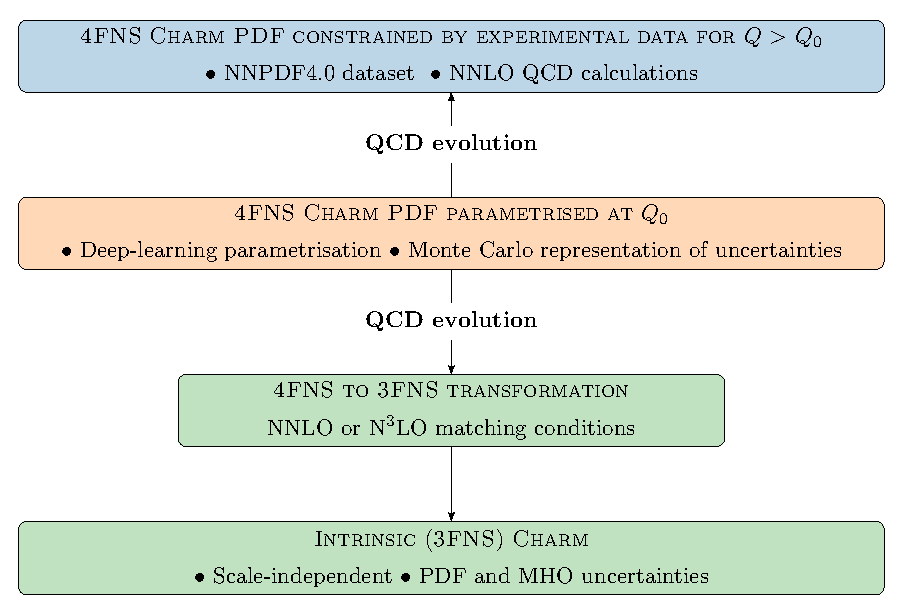
\includegraphics[width=0.8\textwidth]{ch-ic/strategy.pdf}
 \end{center}
\vspace{-0.2cm}
\caption{The 4FNS charm PDF is parametrized  at $Q_0$
  and evolved to all  $Q$, where it is  constrained by the NNPDF4.0
  global dataset. 
  %
 Subsequently, it is transformed to the 3FNS where (if nonzero) it
 provides the intrinsic charm component.
  \label{fig:ic/strategy}
}
\end{figure}
%%%%%%%%%%%%%%%%%%%%%%%%%%%%%%%%%%%%%%%%%%%%

\paragraph{Global QCD analysis.}
%
The 4FNS charm PDF and its associated
uncertainties is determined by means of a global QCD analysis
within the NNPDF4.0 framework.
%
All PDFs, including the charm PDF, are  parametrized at $Q_0=1.65$ GeV in 
a model-independent manner using a neural network, which is fitted to data using 
supervised machine learning techniques.
The Monte Carlo replica method
is deployed to ensure a faithful uncertainty estimate.
%
Specifically, we express the 4FNS total charm PDF ($c^+=c+\bar{c}$)  in terms of the output neurons associated to the quark singlet $\Sigma$ and non-singlet $T_{15}$
distributions, see Sect.~3.1 of~\cite{Ball:2021leu}, as
\begin{equation}
\label{eq:ic/fitted_charm_param}
xc^+(x,Q_0;{\boldsymbol \theta}) =
\left( x^{\alpha_{\Sigma}}(1-x)^{\beta_{\Sigma}} \textrm{ NN}_{\Sigma}(x,{\boldsymbol \theta})-
x^{\alpha_{T_{15}}}(1-x)^{\beta_{T_{15}}} \textrm{ NN}_{T_{15}}(x,{\boldsymbol \theta})
\right)/4 \, ,
\end{equation}
where $\textrm{
  NN}_{i}(x,{\boldsymbol \theta})$ is the $i$-th output neuron of a
neural network with input $x$ and  parameters ${\boldsymbol \theta}$,
and 
$\left( \alpha_i,\beta_i\right) $ are
preprocessing exponents.
%
A crucial feature of Eq.~(\ref{eq:fitted_charm_param}) is that no \textit{ ad hoc} specific model assumptions are used:ic/ the shape and size of $xc^+(x,Q_0)$ are entirely determined from experimental data.
%
Hence, our determination of the 4FNS fitted charm PDF, and thus of the intrinsic charm, is unbiased.
%

%%%%%%%%%%%%%%%%%%%%%%%%%%%%%%%%%%%%%%%%%%%%
\begin{figure}[t]
\begin{center}
  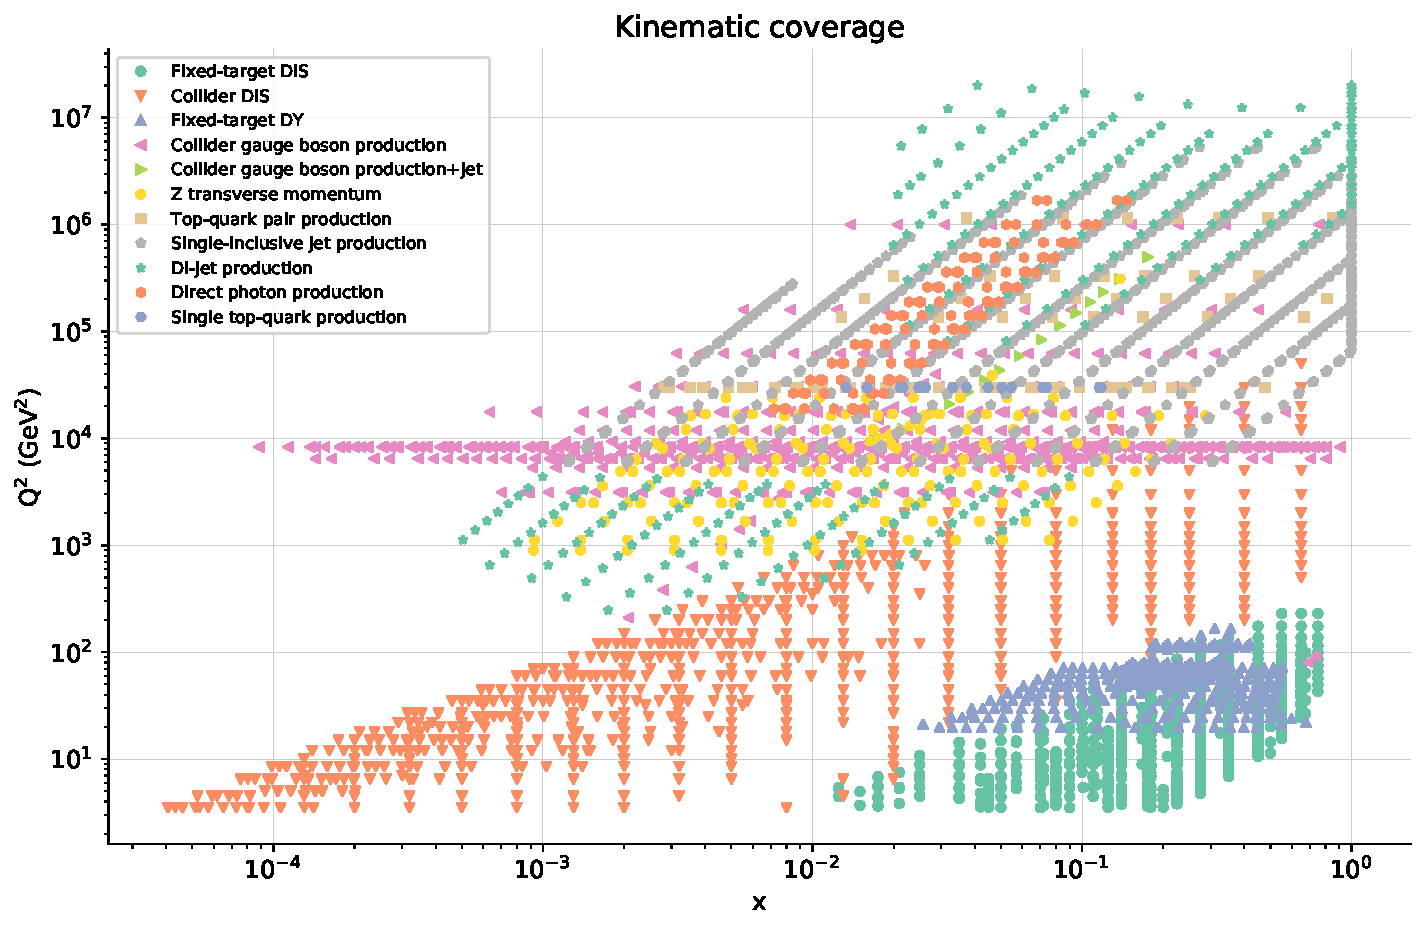
\includegraphics[width=1.0\textwidth]{ch-ic/kinplot.pdf}
 \end{center}
\vspace{-0.8cm}
\caption{The kinematic coverage in the $(x,Q)$ plane
  covered by the 4618 cross-sections used for the
  determination of the charm PDF in the present work.
  %
  These cross-sections have been classified into the main different
  types of processes entering the global analysis.
  \label{fig:ic/kinplot}
}
\end{figure}
%%%%%%%%%%%%%%%%%%%%%%%%%%%%%%%%%%%%%%%%%%%%

The neural network parameters ${\boldsymbol \theta}$ in
Eq.~(\ref{eq:ic/fitted_charm_param})
are determined by fitting an extensive global dataset that consists of 4618 
cross-sections from a wide range of different processes, measured over
the years in a variety of fixed-target and collider experiments  (see~\cite{Ball:2021leu} for a complete list).
%
Fig.~\ref{fig:ic/kinplot} displays the kinematic coverage in the $(x,Q)$ plane
covered by these cross-sections, where $Q$ is
the  scale, and  $x$ is
the parton momentum fraction that correspond to leading-order kinematics.
%
Many of these processes provide direct or indirect sensitivity 
to the charm content of the proton.
%
Particularly important constraints come from $W$ and $Z$ production from 
ATLAS, CMS, and LHCb as well as from
neutral and charged current deep-inelastic 
scattering (DIS) structure functions from HERA.
%
The 4FNS  PDFs at the input scale $Q_0$ are related
to experimental measurements at $Q \not =Q_0$ by means of NNLO QCD calculations, including
the FONLL-C general-mass scheme for DIS~\cite{Forte:2010ta} generalized to 
allow for fitted charm~\cite{Ball:2015tna}.

We have verified (see
SI Sects.~\ref{app:charm_stability_4fns} and~\ref{app:ic/charm_stability_3fns}) that the
determination of 4FNS charm PDF Eq.~(\ref{eq:ic/fitted_charm_param}) and
the ensuing 3FNS intrinsic charm PDF are  stable upon variations
of methodology (PDF parametrization basis), input dataset, and values
of Standard Model parameters (the charm mass).
We have also studied the stability of our results upon replacing the
current NNPDF4.0 methodology~\cite{Ball:2021leu} with the previous
NNPDF3.1 methodology~\cite{NNPDF:2017mvq}. It turns out that results
are  perfectly consistent. Indeed, the old methodology leads to somewhat larger
uncertainties, corresponding to a moderate reduction of the local statistical
significance for intrinsic charm, and to a central value which is
within the smaller  error band of our current result.


A determination in which the vanishing of intrinsic charm is
imposed has also been performed.
%
In this case, the fit quality significantly
deteriorates: the values of the $\chi^2$ per data point of 1.162,
1.26, and 1.22 for total, Drell-Yan, 
and neutral-current DIS data respectively, found when fitting charm, are 
increased to 1.198, 1.31, 1.28 when the vanishing of intrinsic charm
is imposed.
%
The absolute worsening of the total $\chi^2$ when the vanishing of intrinsic charm is imposed is therefore
of 166 units, corresponding to
a $2\sigma$ effects in units of $\sigma_{\chi^2}= \sqrt{2n_\textrm{ dat}}$.

\paragraph{Calculation of the 3FNS charm PDF.}
%
The Monte Carlo representation of the probability distribution associated to
the 4FNS charm PDF determined by the global
analysis contains an intrinsic component mixed with a perturbatively
generated contribution, with the latter
becoming larger in the $x\lsim 0.1$ region as the scale $Q$ is increased.
%
In order to extract the intrinsic component, 
we transform PDFs to the 3FNS at the scale $Q_c=m_c=1.51$~GeV using
\textsc{\small EKO}, a novel \textsc{\small Python} open source
PDF evolution framework (see  SI Sect.~\ref{app:ic/eko}).
%
In its current implementation, \textsc{\small EKO} performs  QCD 
evolution of PDFs to any scale
up to NNLO. For
the sake of the current analysis, N$^3$LO matching conditions have also
been implemented, by 
using  the results
of~\cite{Bierenbaum:2009zt,Bierenbaum:2009mv,Ablinger:2010ty,Ablinger:2014vwa,Ablinger:2014uka,Behring:2014eya,Ablinger_2014,Ablinger:2014nga,Blumlein:2017wxd}
for $\mathcal{O}(\alpha_s^3)$ operator matrix elements~
so that the direct and inverse transformations from the 3FNS to the
4FNS can be performed at one order
higher.
%
The N$^3$LO contributions to the matching conditions are a subset of
the full N$^3$LO terms that would be required to perform a PDF determination
 to one higher perturbative order, and would
also include currently unknown
N$^3$LO contributions to QCD evolution. Therefore, our results have 
NNLO accuracy and we can only use the  N$^3$LO contributions to the
 $\mathcal{O}(\alpha_s^3)$ corrections to the
heavy quark matching
matching conditions as a way to estimate the 
the size of the missing higher orders. 
Indeed, these corrections have a very 
significant impact on the
perturbatively generated component, see SI Sect.~\ref{app:ic/consistency}.
%
They become large for $x \lsim 0.1$, which coincides with the region
dominated by the perturbative component of the charm PDF,
  and are relatively small for the valence region
  where intrinsic charm dominates.
  
\paragraph{$Z$ production in association with charm-tagged jets.}
%
The production of $Z$ bosons in association with charm-tagged jets (or alternatively,
with identified $D$ mesons) at the LHC is directly sensitive to the charm content
of the proton via the dominant $gc \to Zc$ partonic scattering process.
%
Measurements of this process at  the forward rapidities covered by the
LHCb acceptance provide access to the large-$x$ region where the intrinsic 
contribution is expected to dominate.
%
This is in contrast with the corresponding measurements from ATLAS and CMS,
which only become sensitive to intrinsic charm
at rather larger values of $p_T^Z$ than those
currently accessible experimentally.

We have obtained  theoretical predictions for $Z$+charm production
at LHCb with NNPDF4.0, based on
NLO QCD calculations using
\textsc{\small POWHEG-BOX} 
interfaced to \textsc{\small Pythia8}
with the Monash 2013 tune for showering,
hadronization, and underlying event.
%
Acceptance requirements and event selection follow the LHCb analysis,
where in particular charm jets are defined as those anti-$k_T$ $R=0.5$ jets
containing a reconstructed charmed hadron.
%
The ratio between $c$-tagged and untagged $Z$+jet events can then
be compared with the LHCb measurements
\begin{equation}
  \mathcal{R}_j^c(y_Z) \equiv \frac{N(c~\textrm{ tagged~jets};y_Z)}{ 
    N(\textrm{ jets};y_Z)} =
  \frac{\sigma(pp\to Z+\textrm{ charm~ jet};y_Z)}{\sigma(pp \to Z+\textrm{ jet};y_Z)} \, ,
\end{equation}
as a function of the $Z$ boson rapidity $y_Z$ (see SI Sect.~\ref{sec:ic/zcharm} for details).
%
The more forward the rapidity $y_{Z}$, the higher the values of the charm
momentum $x$ being probed.
%
Furthermore, we have also included the LHCb measurements in the global PDF
determination by means of the Bayesian reweighting (see SI
Sect.~\ref{sec:ic/zcharm}).
